\documentclass[11pt,a4paper]{article}
\usepackage[left=2.5cm,right=2cm, bottom=2cm]{geometry}
\usepackage[utf8]{inputenc}
\usepackage{amsmath}
\usepackage{amsfonts}
\usepackage{amssymb}
\usepackage{amsfonts}
\usepackage{amsmath}
\usepackage{graphicx}
\usepackage{subfigure}
\usepackage{color}
\usepackage{abstract}
\usepackage{float}
\usepackage[toc,page]{appendix}
\usepackage{hyperref}
\usepackage{fancyhdr}
\usepackage{algorithm} 
\usepackage{algpseudocode} 
\usepackage{listings}
\usepackage{xcolor} % for setting colors
% set the default code style
\lstset{
	frame=tb, % draw a frame at the top and bottom of the code block
	tabsize=4, % tab space width
	showstringspaces=false, % don't mark spaces in strings
	numbers=left, % display line numbers on the left
	commentstyle=\color{green}, % comment color
	keywordstyle=\color{blue}, % keyword color
	stringstyle=\color{red} % string color
}

\pagestyle{fancy}
\fancyhf{}
\rhead{\today}
\lhead{\bfseries Alexander Leitner 01525882}
\rfoot{}



\begin{document}
\begin{center}
	\fontsize{24pt}{10pt}\selectfont
	\textsc{\textbf{Computational Science on Many-Core Architectures  Exercise 5}}
\end{center}
\section*{Example 1 Inclusive and Exclusive Scan (4 Points)}
\subsection*{a)}
\begin{center}
	
	\begin{minipage}[t]{0.40\textwidth}
		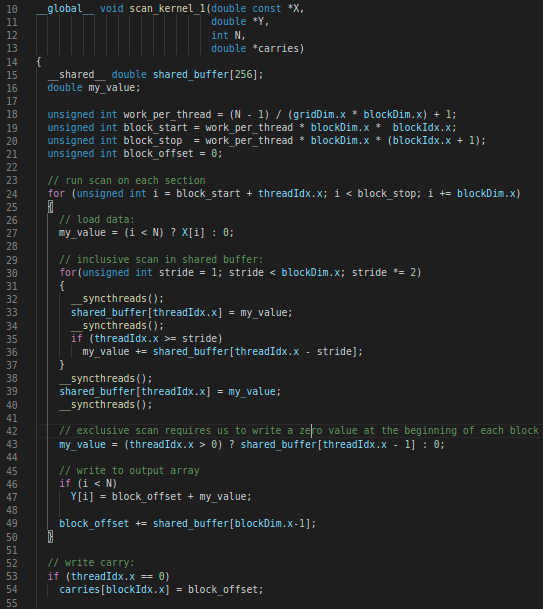
\includegraphics[width=\textwidth]{Bilder/Ex5_1_1}
	\end{minipage}
	
\end{center}
For the first kernel "kernel\_1" and simulate it with 4 blocks and 6 threads per block.\\
Begin with line 24: the for loop iterates over the values X which belong to the block.\\
At the end of the for loop $\rightarrow$ write the temporary result of the scan into a vector Y and the offset stored in block\_offset. At the end of the kernel every block contains it scanned value and the vector for the next step.
\begin{center}
	
	\begin{minipage}[t]{0.40\textwidth}
		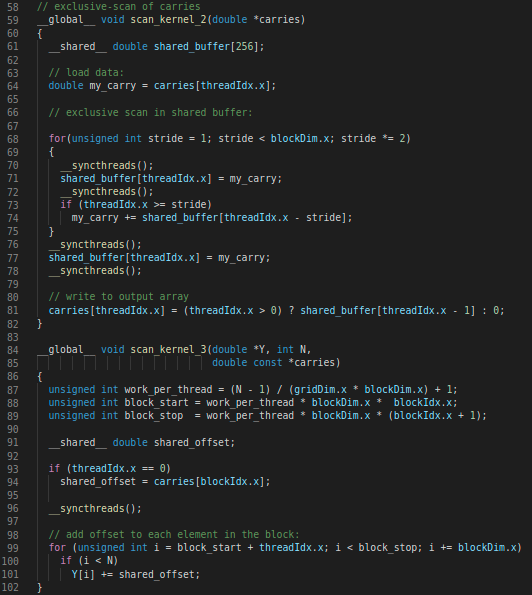
\includegraphics[width=\textwidth]{Bilder/Ex5_1_2}
	\end{minipage}
	
\end{center}
\newpage 
	
\begin{minipage}[t]{0.5\textwidth}
	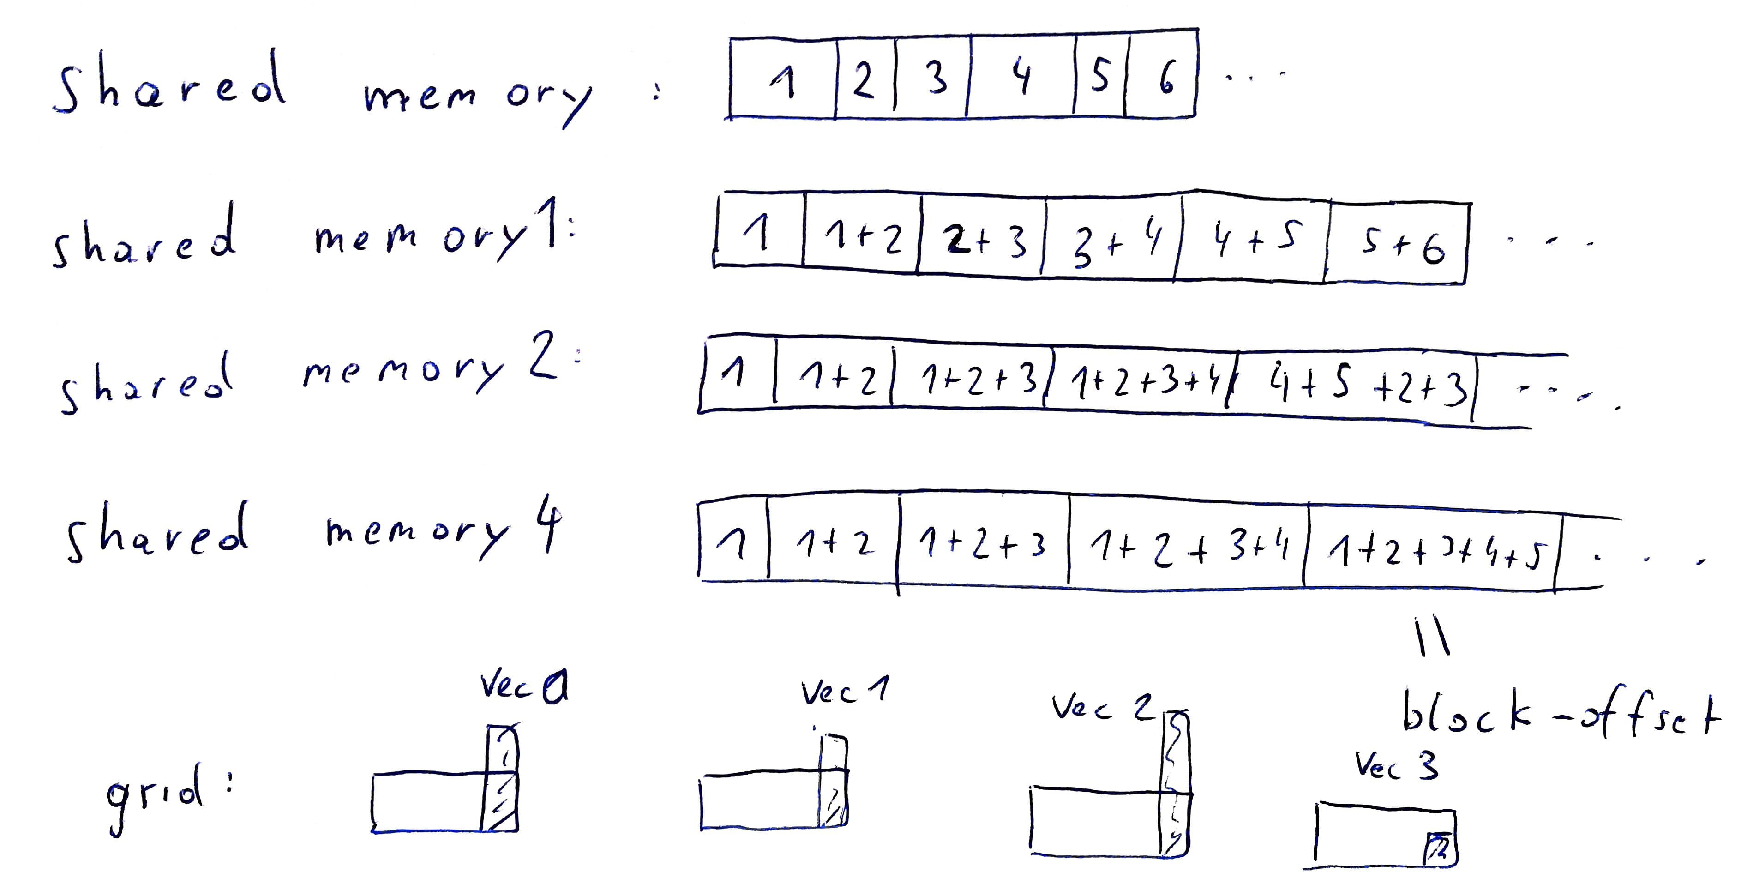
\includegraphics[width=\textwidth]{Bilder/Ex5_1_3}
\end{minipage}
\begin{minipage}[t]{0.27\textwidth}
	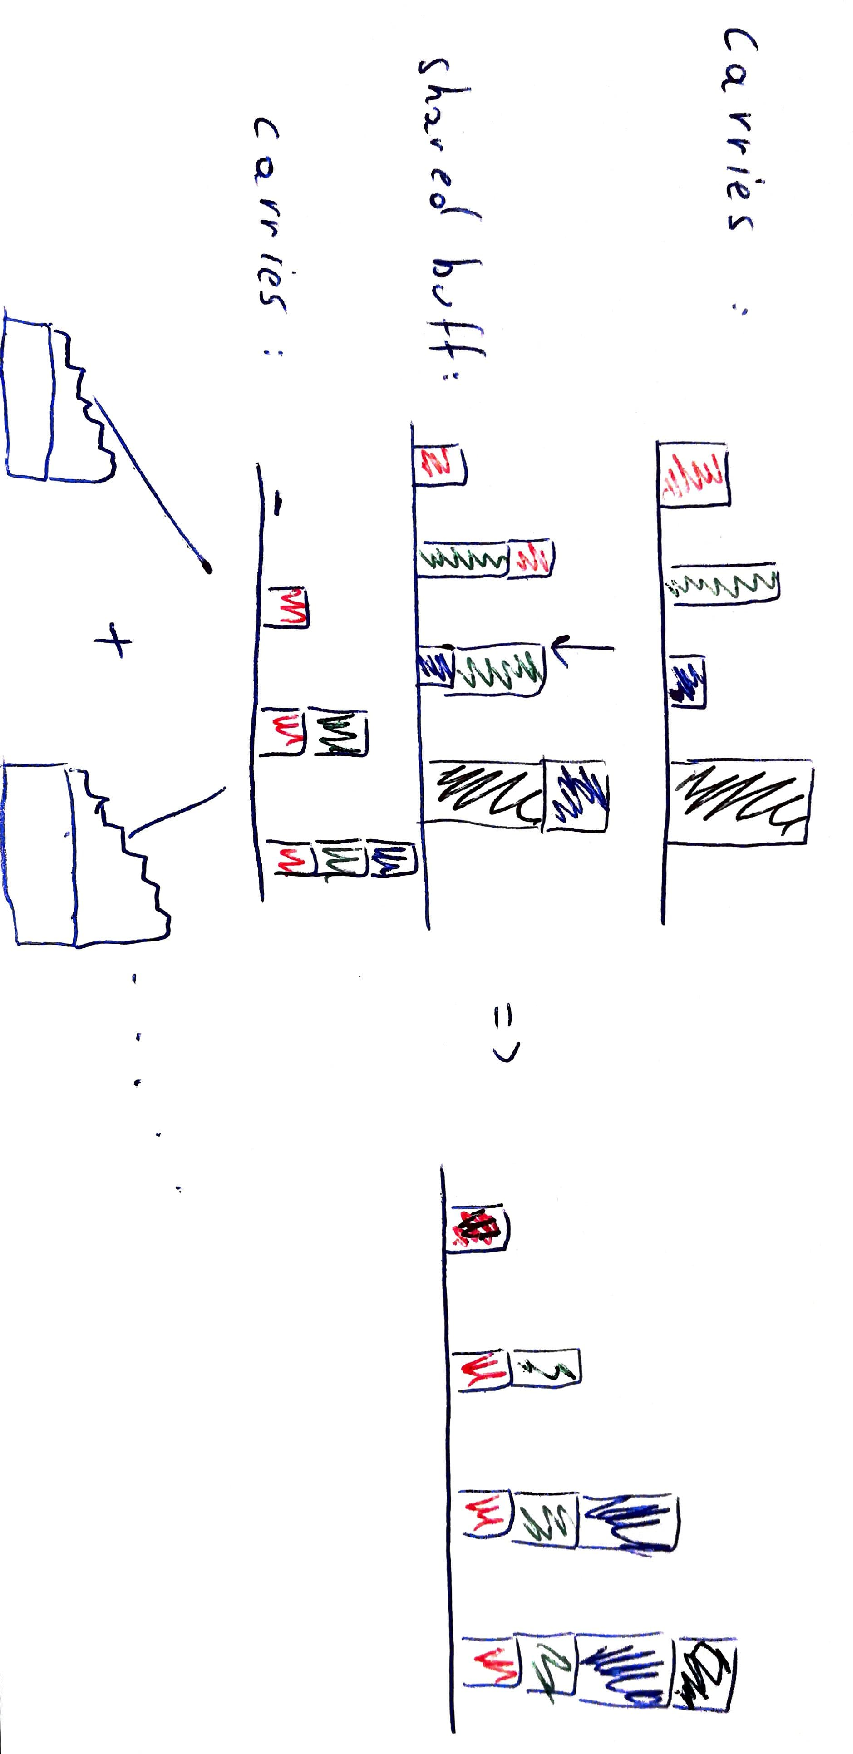
\includegraphics[width=\textwidth,angle=90]{Bilder/Ex5_1_4}
\end{minipage}

\subsection*{b)}
\begin{lstlisting}[language=C++, caption={kernel for inclusive\_scan)}]
__global__ void Inclusive(double *Y, int N, const double *X)
{
	for (int i = blockDim.x * blockIdx.x + threadIdx.x; i < N-1; 
	i += gridDim.x * blockDim.x) 
	{
		Y[i] = Y[i+1];
	}
	if (blockDim.x * blockIdx.x + threadIdx.x == 0)
		// First step: Scan within each thread group and write carries
	scan_kernel_1<<<num_blocks, threads_per_block>>>(input, output, N, carries);
	
	// Second step: Compute offset for each thread group 
	(exclusive scan for each thread group)
	scan_kernel_2<<<1, num_blocks>>>(carries);
	
	// Third step: Offset each thread group accordingly
	scan_kernel_3<<<num_blocks, threads_per_block>>>(output, N, carries);
	
	// Make inclusive
	makeInclusive<<<num_blocks, threads_per_block>>>(output, N, input);
	
	cudaFree(carries);
	{
		Y[N-1] += X[N-1];
	}		
}

void exclusive_scan(double const * input, double* output, int N)
{
	int num_blocks = 512;
	int threads_per_block = 512;

	double *carries;
	cudaMalloc(&carries, sizeof(double) * num_blocks);

	// First step: Scan within each thread group and write carries
	scan_kernel_1<<<num_blocks, threads_per_block>>>(input, output, N, carries);
	
	// Second step: Compute offset for each thread group 
	(exclusive scan for each thread group)
	scan_kernel_2<<<1, num_blocks>>>(carries);
	
	// Third step: Offset each thread group accordingly
	scan_kernel_3<<<num_blocks, threads_per_block>>>(output, N, carries);
	
	// Make inclusive
	makeInclusive<<<num_blocks, threads_per_block>>>(output, N, input);
	
	cudaFree(carries);
}
\end{lstlisting}
\subsection*{c)}
Only nessesary to remove the folloing code snipped:
\begin{lstlisting}[language=C++, caption={kernel for inclusive\_scan)}]
// exclusive scan requires us to write a zero value
at the beginning of each block
my_value = (threadIdx.x > 0) ? shared_buffer[threadIdx.x - 1] : 0;
\end{lstlisting}
\subsection*{d)}
\begin{center}
	
	\begin{minipage}[t]{0.70\textwidth}
		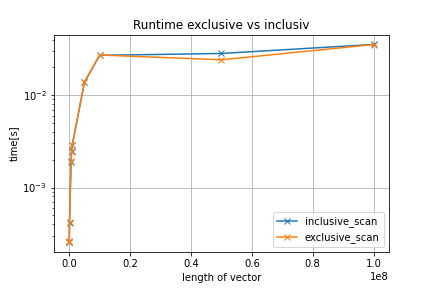
\includegraphics[width=\textwidth]{Bilder/runtime_excl_vs_inclu}
	\end{minipage}
	
\end{center}
There is bassicaly no differences.
\newpage
\section*{2 Poisson equation (5 Points)}
First I have to change all row\_offsets, indices to an int datatype because there was an error with the matching datatype for the residual\_norm function in "poisson2D.hpp".
\subsection*{a)}
\begin{lstlisting}[language=C++, caption={kernel for serching for zeros)}]
__global__ void count_nonzero_entries(int* row_offsets, int N, int M) {
	for(int row = blockDim.x * blockIdx.x + threadIdx.x; row < N * M;
	 row += gridDim.x * blockDim.x) {
		int nnz_for_this_node = 1;
		int i = row / N;
		int j = row % N;
		
		if(i > 0) nnz_for_this_node += 1;
		if(j > 0) nnz_for_this_node += 1;
		if(i < N-1) nnz_for_this_node += 1;
		if(j < M-1) nnz_for_this_node += 1;
		
		row_offsets[row] = nnz_for_this_node;
	}
}
\end{lstlisting}
\subsection*{b)}
Again changed the double const *input to a int const * input.
\begin{lstlisting}[language=C++, caption={given exclusive scan)}]
void exclusive_scan(int const * input,
int       * output, int N)
{
	int num_blocks = 512;
	int threads_per_block = 512;
	
	int *carries;
	cudaMalloc(&carries, sizeof(int) * num_blocks);
	
	// First step: Scan within each thread group and write carries
	scan_kernel_1<<<num_blocks, threads_per_block>>>(input, output, N, carries);
	
	// Second step: Compute offset for each thread group (exclusive scan for each thread group)
	scan_kernel_2<<<1, num_blocks>>>(carries);
	
	// Third step: Offset each thread group accordingly
	scan_kernel_3<<<num_blocks, threads_per_block>>>(output, N, carries);
	
	cudaFree(carries);
}
\end{lstlisting}
\subsection*{c)}
\begin{lstlisting}[language=C++, caption={assemble the matrix A)}]
__global__ void assemble_A_GPU(double* values, int* columns, int* row_offsets, int N, int M) 
{
	for(int row = blockDim.x * blockIdx.x + threadIdx.x; 
	row < N*M; row += gridDim.x * blockDim.x) 
	{
		int i = row / N;
		int j = row % N;
		int counter = 0;
		
		if ( i > 0) 
		{
			values[(int)row_offsets[row] + counter] = -1;
			columns[(int)row_offsets[row] + counter] = (i-1)*N+j;
			counter++;
		}
		
		if ( j > 0) 
		{
			values[(int)row_offsets[row] + counter] = -1;
			columns[(int)row_offsets[row] + counter] = i*N+(j-1);
			counter++;
		}
		
		values[(int)row_offsets[row] + counter] = 4;
		columns[(int)row_offsets[row] + counter] = i*N+j;
		
		counter++;
		
		if ( j < M-1) 
		{
			values[(int)row_offsets[row] + counter] = -1;
			columns[(int)row_offsets[row] + counter] = i*N+(j+1);
			counter++;
		}
		if ( i < N-1) 
		{
			values[(int)row_offsets[row] + counter] = -1;
			columns[(int)row_offsets[row] + counter] = (i+1)*N+j;
			counter++;
		}
	}
}
\end{lstlisting}
\newpage
\subsection*{d)}
Just adapt the GD program that you gave us and changed the names from the row\_offsets.\\
Code is in the appendix in the mail.
\subsection*{e)}
Simply replace the conditions for the loop in the assembling kernel with this.\\
Code is in the appendix in the mail.
\begin{lstlisting}[language=C++, caption={kernel for serching for zeros)}]
for(int row = 0; row < N*M; row++)
\end{lstlisting}

\begin{minipage}[t]{0.49\textwidth}
	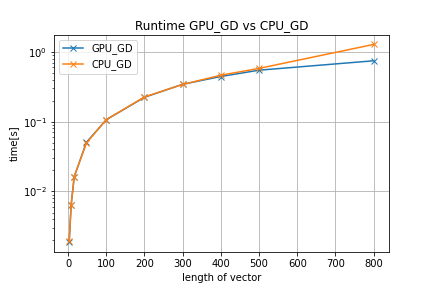
\includegraphics[width=\textwidth]{Bilder/runtime_GPU_vs_CPU}
\end{minipage}
\begin{minipage}[t]{0.49\textwidth}
	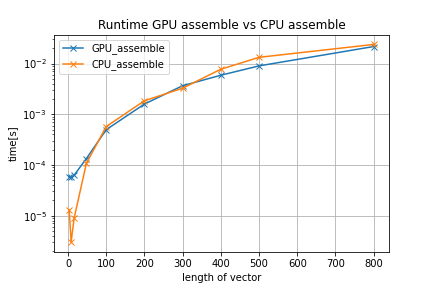
\includegraphics[width=\textwidth]{Bilder/runtime_assemble_GPU_vs_assemble_CPU}
\end{minipage}

\noindent
In total the differences are not that much. Maybe for higher dimensions of the matrix $A$ but I got an SEGMENTATION FAULT at a certain point of the benchmark $N > 800$. I tried to change int into a long int but then I got also some errors. I think the difference should be much higher for bigger dimensions of $A$.
\newpage
\subsection*{f) Bonus point}
Very ineffective way to get the results for the plotting. The two for loops outputs the first line of the solution matrix. 
\begin{lstlisting}[language=C++, caption={kernel for serching for zeros)}]
int ck = 0; 
for (int i = 0; i < N/max; i++)
{
	for (int j = 0; j < N/max; j++)
	{
		std::cout << solution[ck] << "," << std::endl;
		ck = ck + 1;
	}
	std::cout << " " << std::endl;  
	std::cout << " " << std::endl;
	std::cout << " " << std::endl;
	std::cout << " " << std::endl;
	std::cout << " " << std::endl;
}
\end{lstlisting}
I copied the output by hand in python and plot it with the function "heat\_map". The dimension of the solution is $16\times16$ so in total 256 unknowns. The result looks nice. It is obviously the solution to the poisson equation.   
\begin{center}
	
	\begin{minipage}[t]{1\textwidth}
		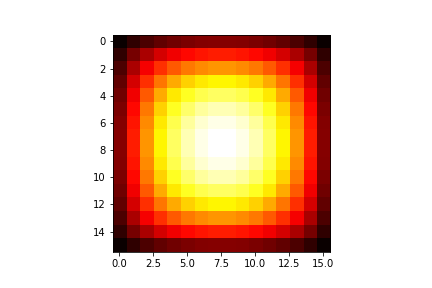
\includegraphics[width=\textwidth]{Bilder/solution_16x16}
	\end{minipage}
	
\end{center}
The color bar on the side represents the amplitude of the solution.
Where $N$ and $M$ are the cordinates of the solution matrix. In our case is the unite square given in the matrix assemble function.
 
\end{document}